\section{Configuration}

\subsection{Common}

\subsubsection{Main}

\begin{figure}[H]
    \center
      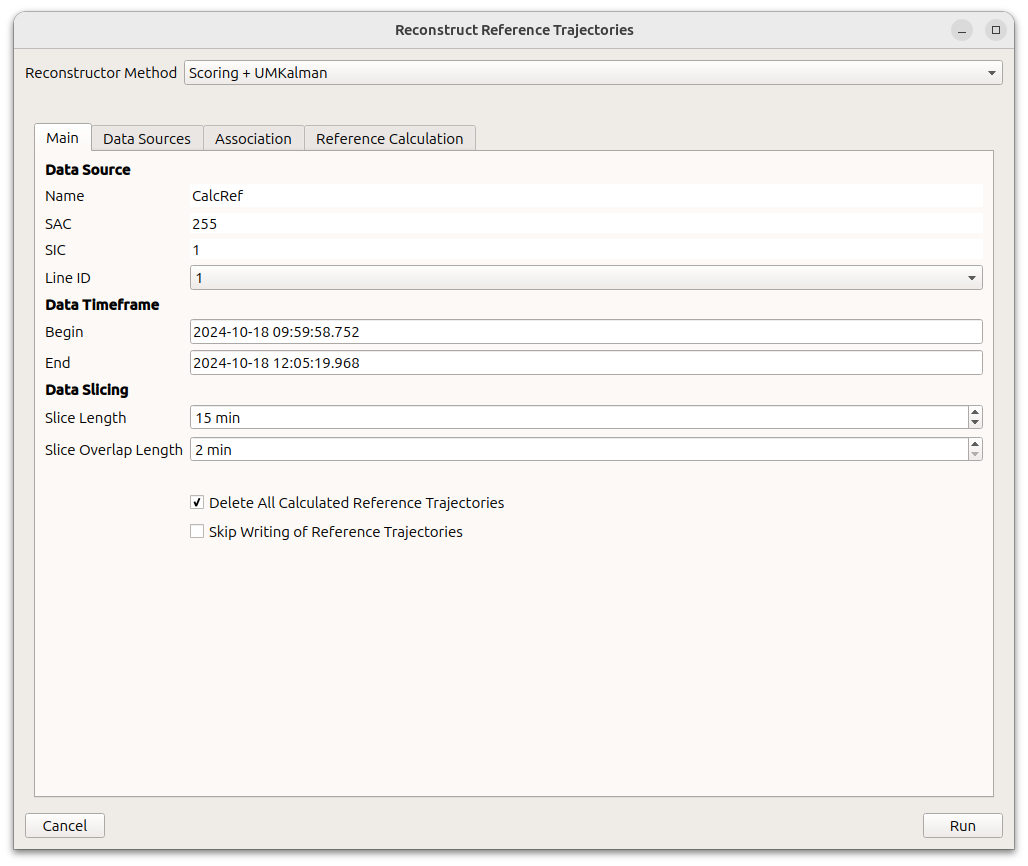
\includegraphics[width=16cm]{figures/dialog_main.png}
    \caption{Calculate References Main}
\end{figure}

In the main tab, the following parameters can be set:

\begin{itemize}
\item Data Source: Data source to be created for calculated references
    \begin{itemize}
    \item Name, SAC, SIC: Data source parameters
    \item Line ID: Line ID to be used
    \end{itemize}
\item Data Timeframe: Time window of data to be processed
    \begin{itemize}
    \item Begin / End timestamps
    \end{itemize}
\item Data Slicing: Time slice sizes
    \begin{itemize}
    \item Slice Length: Duration of a time slice
    \item Slice Overlap Length: Duration of an overlap region to "glue" slices together
    \end{itemize}
\item Delete All Calculated Reference Trajectories: If active, all previous calculated references are deleted
\item Skip Writing of Reference Trajectories: If active, calculated references are not written into the database, only the associations
\end{itemize}
\ \\

\subsubsection{Data Sources}

\begin{figure}[H]
    \center
      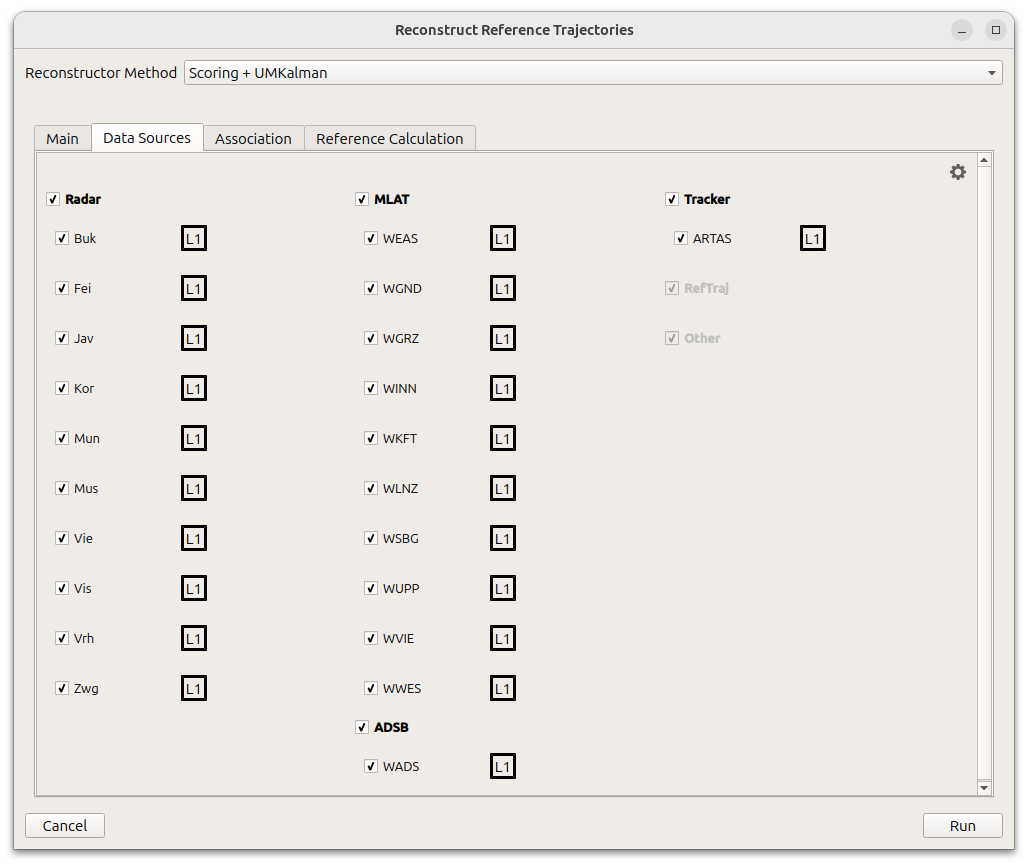
\includegraphics[width=16cm]{figures/dialog_data_sources.png}
    \caption{Calculate References Data Sources}
\end{figure}

In this tab, the data sources to contribute to the calculated references can be selected. \\

Please \textbf{note} that de-selected data sources are still associated, but only their target report positions do not contribute to the references.

\subsection{Scoring + UMKalman Parameters}

\subsubsection{Association}

\begin{figure}[H]
    \center
      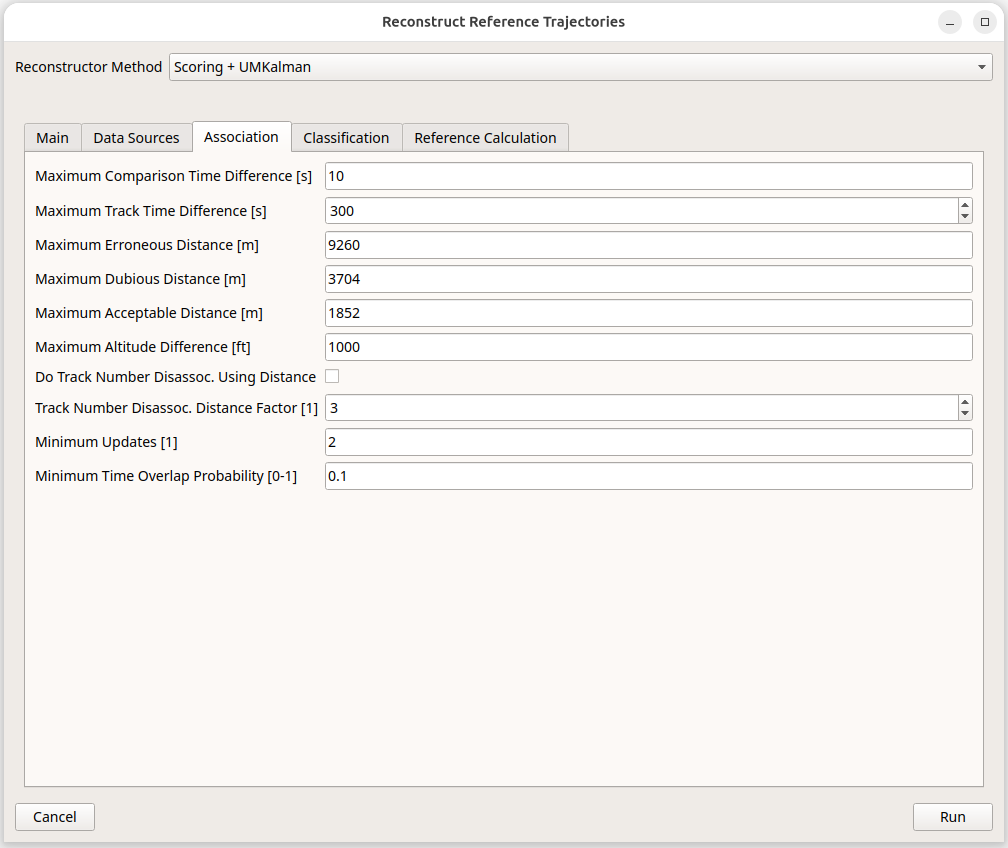
\includegraphics[width=16cm]{figures/dialog_scorum_assoc.png}
    \caption{Scoring + UMKalman Association Parameters}
\end{figure}

In this tab, the association parameters can be set, i.e. the thresholds used to associate target reports to targets, or targets to targets. \\

\begin{table}[H]
  \center
  \begin{tabularx}{\textwidth}{ | l | l | X |}
    \hline
    \textbf{Parameter} & \textbf{Default} &  \textbf{Description} \\ \hline
    Maximum Comparison Time Difference [s] & 15 & Maximum time delta for any code/position comparison \\ \hline
    Maximum Quit Distance [m] & 18520 & Target/target association \\ \hline
    Maximum Dubious Distance [m] & 5556 & Target/target association \\ \hline
    Maximum Acceptable Distance [m] & 1852 & Target/target association \\ \hline
    Maximum Altitude Difference [ft] & 300 & Maximum altitude difference \\ \hline
    Do Track Number Disassoc. Using Distance & false & Whether to disassociated track numbers from targets based on position \\ \hline
    Track Number Disassoc. Distance Factor [1] & 3 & Maximum number of standard deviations distance \\ \hline
    Minimum Updates [1] & 2 & Target/target association \\ \hline
    Minimum Time Overlap Probability [0-1] & 0.1 & Target/target association \\ \hline
  \end{tabularx}
\end{table}

\subsubsection{Reference Calculation}
\label{sec:reconst_scorum_ref_calc} 

\begin{figure}[H]
    \center
      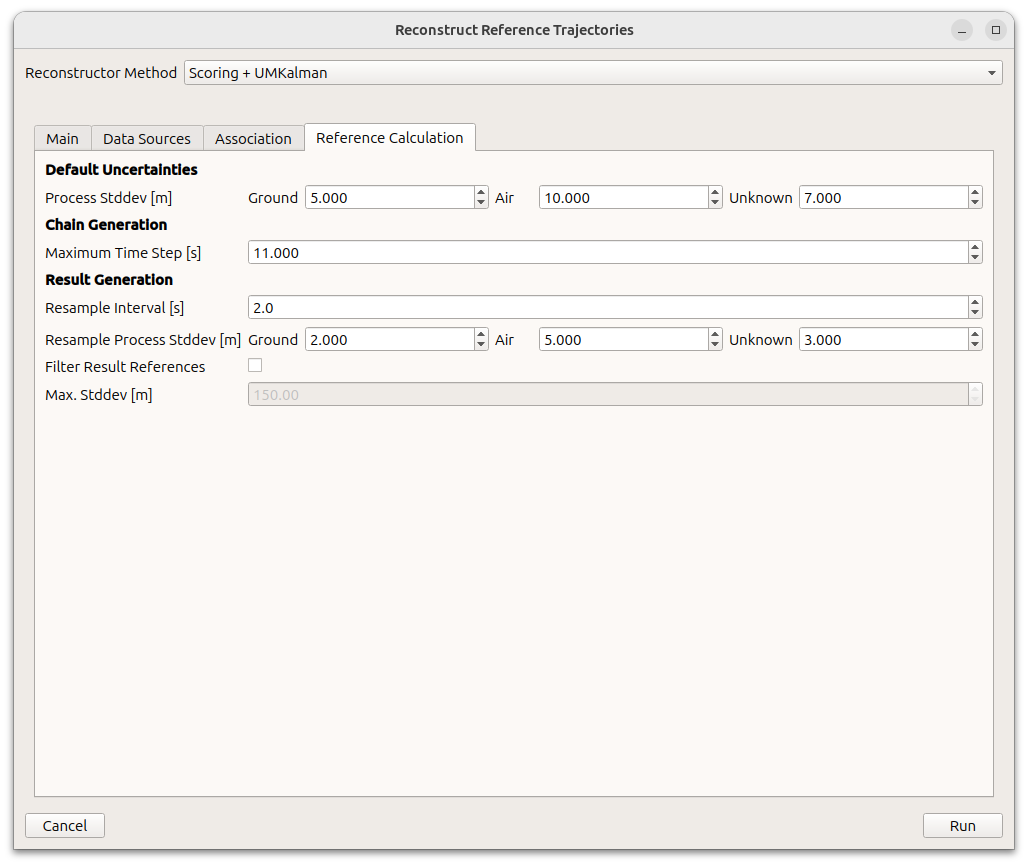
\includegraphics[width=16cm]{figures/dialog_ref_calc.png}
    \caption{Scoring + UMKalman Reconstruction Parameters}
\end{figure}

In this tab, the reference calculation parameters can be set, i.e. the Kalman and reconstruction parameters used for position estimation of the references. \\

\begin{table}[H]
  \center
  \begin{tabularx}{\textwidth}{ | l | l | X |}
    \hline
    \textbf{Parameter} & \textbf{Default} &  \textbf{Description} \\ \hline
    Process Stddev [m] Ground & 3 & Process noise for ground targets \\ \hline
    Process Stddev [m] Air & 10 & Process noise for FL400 targets \\ \hline
    Process Stddev [m] Unknown & 7 & Process noise for targets w/o altitude \\ \hline
    Maximum Time Step [s] & 11 & Re-init reference if no update available within given time \\ \hline
    Resample Interval[s] & 2 & Update interval for the resampled reference trajectories \\ \hline
    Resample Process Stddev [m] Ground & 2 & Resampling process noise for ground targets \\ \hline
    Resample Process Stddev [m] Air & 5 & Resampling process noise for FL400 targets \\ \hline
    Resample Process Stddev [m] Unknown & 3 & Resampling process noise for targets w/o altitude \\ \hline    
    Filter Result References& false & Whether to filter written reference trajectory updates based on maximum position standard deviation \\ \hline
    Max. Stddev [m] & 150 & Maximum position standard deviation \\ \hline
  \end{tabularx}
\end{table}

\subsection{Probabilistic + IMM Parameters}

\subsubsection{Association}

\begin{figure}[H]
    \center
      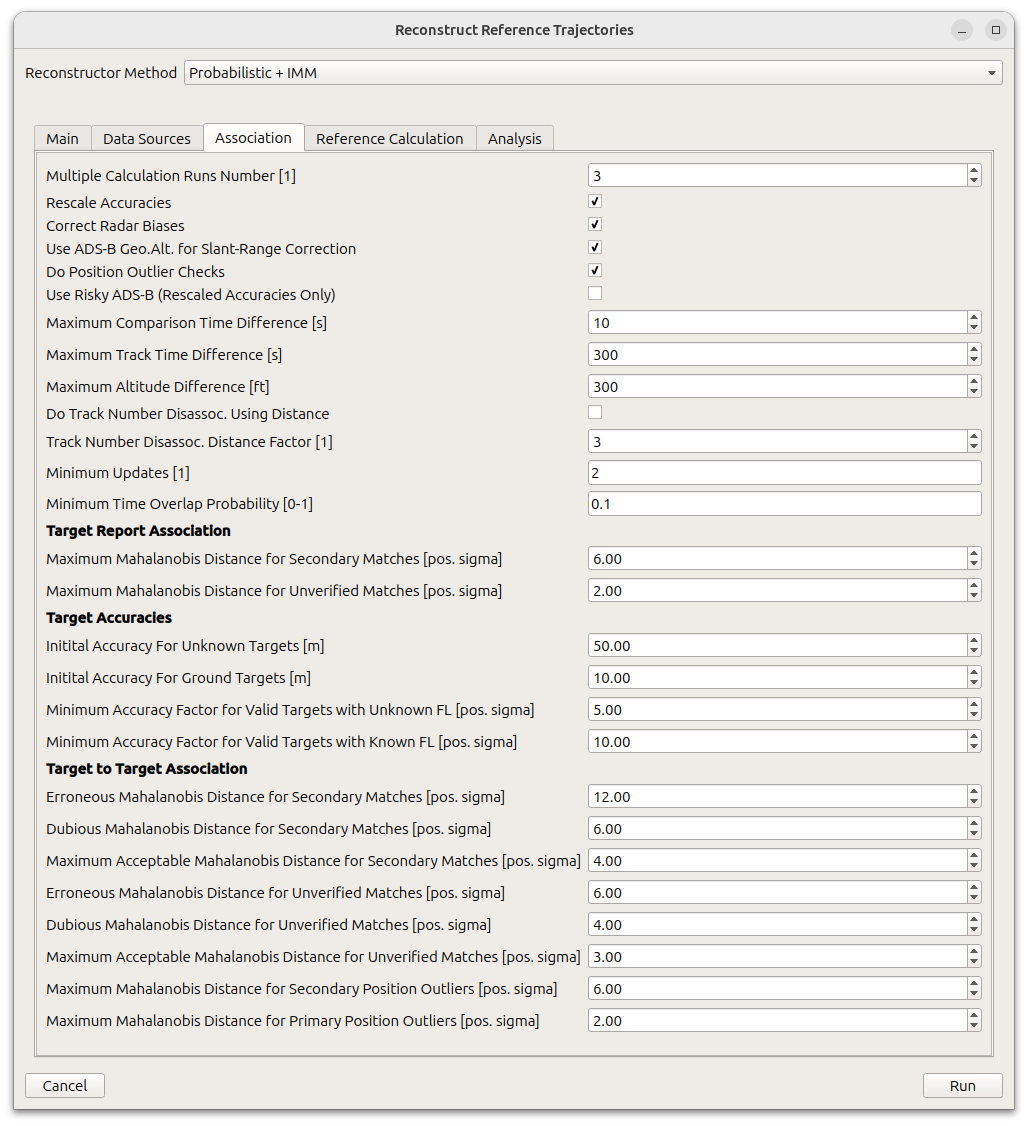
\includegraphics[width=16cm]{figures/dialog_probimm_assoc.png}
    \caption{Probabilistic + IMM Association Parameters}
\end{figure}

Please \textbf{note} that a detailed discussion of the given parameters is out of scope for this user manual. For users with a professional license, a dedicated reconstructor user manual appendix is provided.

\subsubsection{Reference Calculation}

\begin{figure}[H]
    \center
      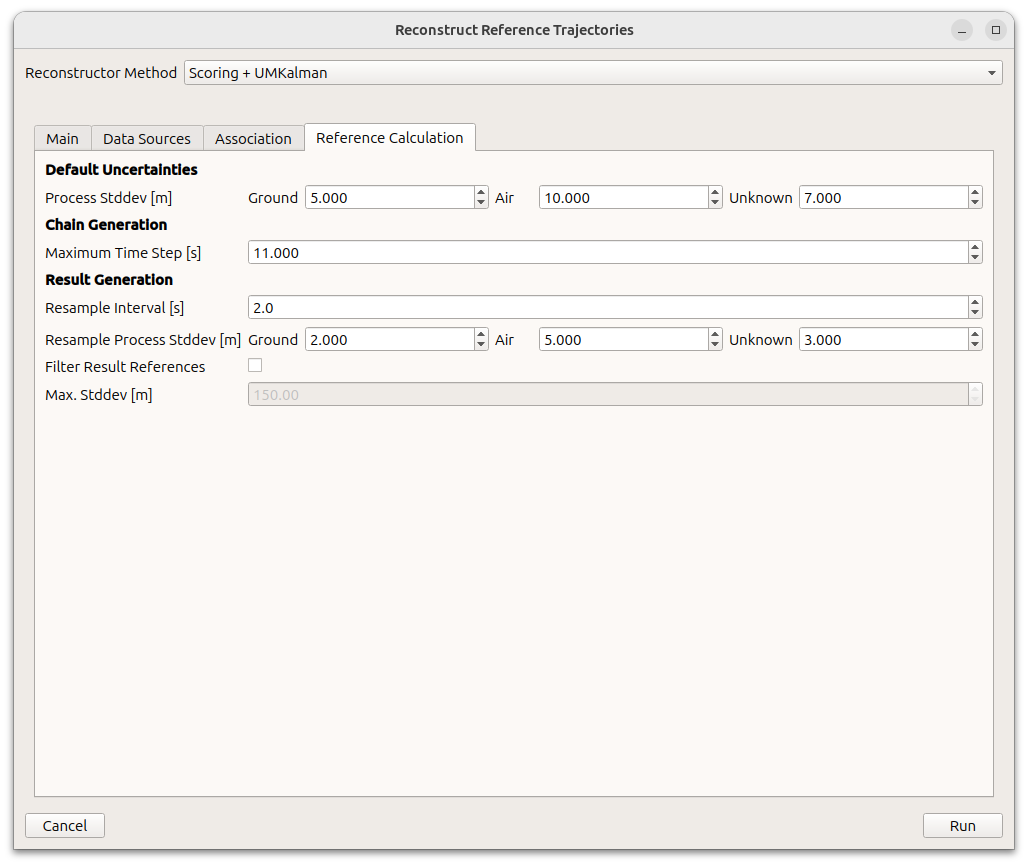
\includegraphics[width=16cm]{figures/dialog_ref_calc.png}
    \caption{Probabilistic + IMM Reconstruction Parameters}
\end{figure}

The given parameters are the same as discussed as with the 'Scoring \& UMKalman' chapter, please refer to \nameref{sec:reconst_scorum_ref_calc} for details.

\subsubsection{Analyse}

\begin{figure}[H]
    \center
      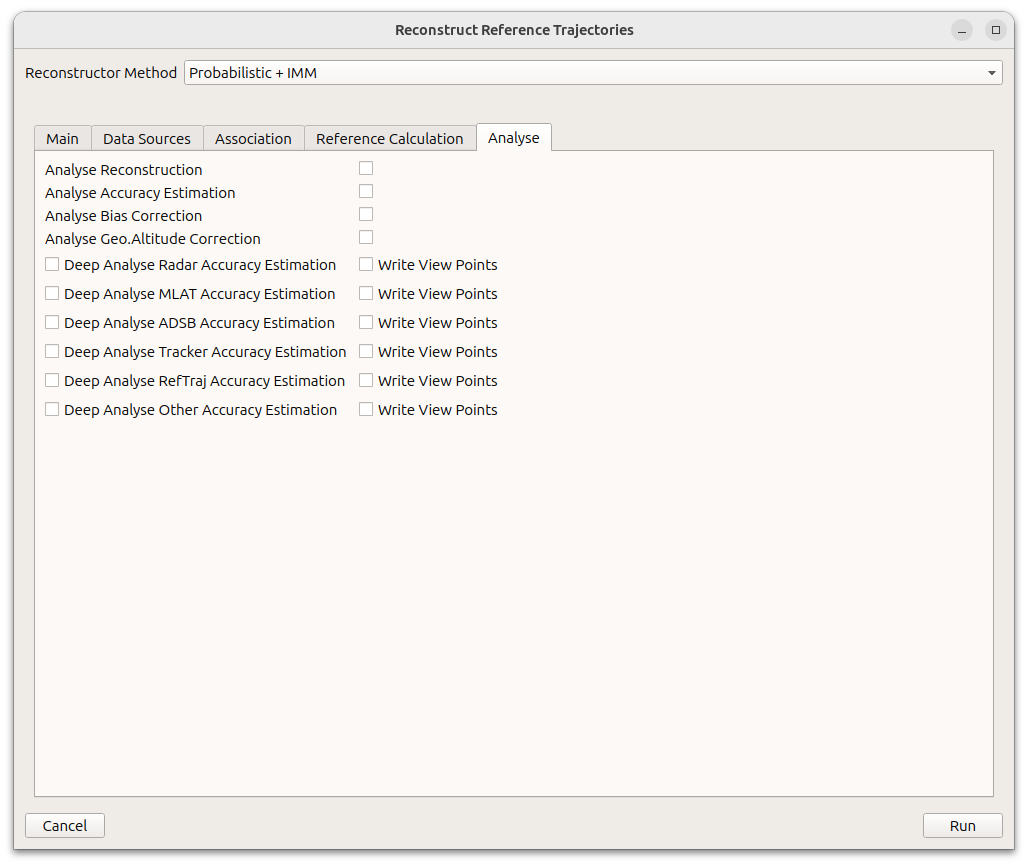
\includegraphics[width=16cm]{figures/dialog_probimm_analyse.png}
    \caption{Probabilistic + IMM Analysis Parameters}
\end{figure}

Please \textbf{note} that a detailed discussion of the given parameters is out of scope for this user manual. For users with a professional license, a dedicated reconstructor user manual appendix is provided.
